\subsection{Future work \label{sec:Fut2}}

\subsubsection{HSL analogue derivatives}

An obvious addition to the library would be the HSL-CipMe conjugate (see \ref{fgr:HL4CipMe}), to enable better comparisons between the triazole-linked and alkyl-linked libraries.

\begin{figure}[H]
	\begin{center}
		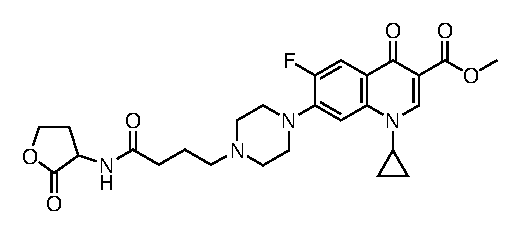
\includegraphics[scale=1]{HL4CipMe}
		\caption{The proposed HSL-CipMe conjugate \compound{cmpd:HL4CipMe}.
		\label{fgr:HL4CipMe}}
	\end{center}
\end{figure}

As methyl ciprofloxacin and its alkyl-linked conjugates had little antibiotic effect, it would be useful to test the carboxylic acid versions of these compounds (see \ref{fgr:fut_cip_anas}). Ideally these would be synthesised directly by hydrolysis of the methyl ciprofloxacin conjugate, but this could potentially cause hydrolysis of the lactone or thiolactone as well. If mild enough hydrolysis conditions could not be found it might be possible to hydrolyse both bonds and then re-form the ring\cite{Witiak1978}. The cyclohexanone conjugate would be best formed by hydrolysis of the cyclohexanol conjugate followed by oxidation of the alcohol to avoid exposing the ketone to extremes of pH.

\begin{figure}[H]
	\begin{center}
		\schemeref[HL4CipMe]{cmpd:HL4Cip}
		\schemeref[SHL4CipMe]{cmpd:SHL4Cip}
		\schemeref[2MeOA4CipMe]{cmpd:2MeOA4Cip}
		\schemeref[3MeOA4CipMe]{cmpd:3MeOA4Cip}
		\schemeref[HOcy5NH4CipMe_RR]{cmpd:HOcy5NH4Cip_RR}
		\schemeref[HOcy5NH4CipMe_SS]{cmpd:HOcy5NH4Cip_SS}
		\schemeref[HOcy6NH4CipMe]{cmpd:HOcy6NH4Cip}
		\schemeref[Ocy6NH4CipMe]{cmpd:Ocy6NH4Cip}
		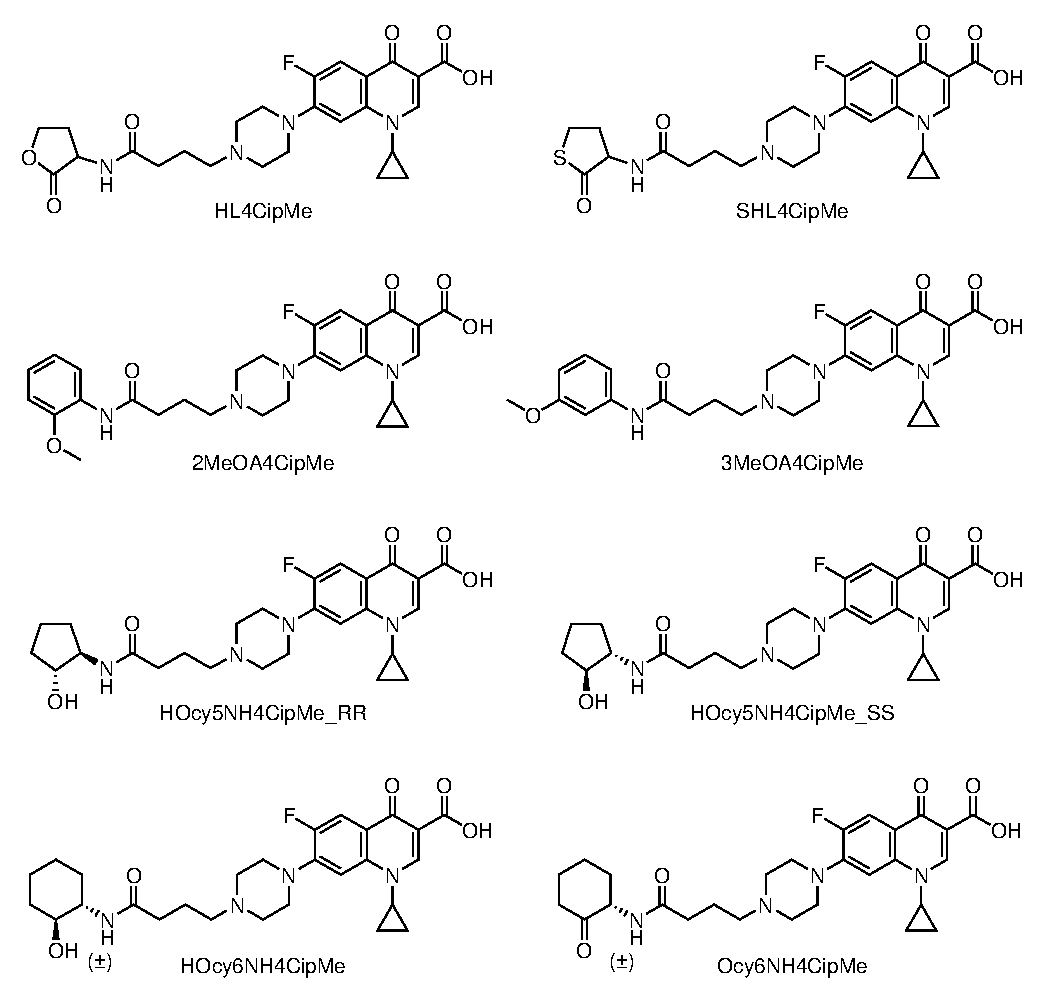
\includegraphics[scale=1]{fut_cip_anas}
		\caption{The proposed HSL analogue-Cip conjugates.
		\label{fgr:fut_cip_anas}}
	\end{center}
\end{figure}

A selection head groups which could be used in future conjugates are shown in \ref{fgr:fut_heads}. These have all been shown to modulate HSL-mediated quorum sensing as part of acyl-HSLs\cite{Smith2003a,Welch2005,Ishida2007,Olsen2002,Smith2003,Hodgkinson2012a,Marsden2010}. The most obvious targets are the cyclopentanone derivatives, as this could be synthesised from the alcohols above. The aniline, pyridine, quinoline and cyclopentyl amine head groups are commercially available and hence derivatives of these could be easily obtained. The 3- and 4-substituted HSL analogues require synthesis, but a route has been devised\cite{Olsen2002}.

\begin{figure}[H]
	\begin{center}
		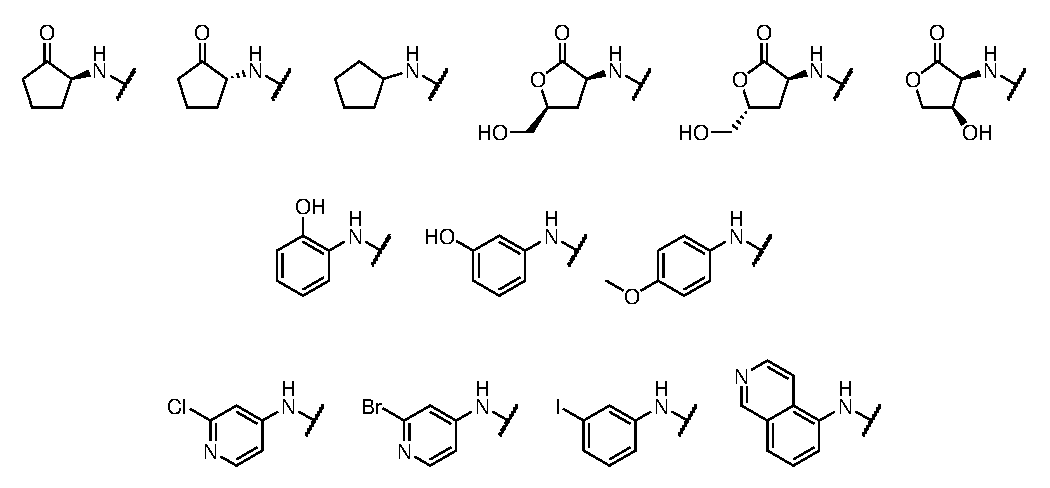
\includegraphics[scale=1]{fut_heads}
		\caption{HSL analogue head groups for use in future conjugates.
		\label{fgr:fut_heads}}
	\end{center}
\end{figure}

\subsubsection{Biology}

The most important next step is the repetition of the biofilm inhibition and dispersal assays with better control over evaporation. 
This can be achieved in a low-tech but reliable manner by placing the sealed plates (without the plastic plate lids) inside a high-sided, open plastic box lined with damp tissue paper.

It is worth noting that Ganguly \textit{et al.} used LIVE/DEAD$^{\tiny{\textregistered}}$ \textit{Bac}Light$^{\tiny{\texttrademark}}$ staining and confocal microscopy to image their biofilms, whereas so far we have used crystal violet staining. Crystal violet does not differentiate between live and dead cells, and so does not pick up on how many cells have been killed within the biofilm but stayed adhered to the plate (their confocal microscopy results do however show a decrease in biofilm thickness so it should be possible to detect this using crystal violet).

We do not have access to a confocal microscope on which we can use \textit{P. aeruginosa}, but alternative stains which show cell viability could be used. Peeters \textit{et al.}\cite{Peeters2008} evaluated six assays used for the quantification of biofilms and recommended fluorescein diacetate or resazurin viability assays for the quantification of live cells in \textit{P. aeruginosa} biofilms.

Given the interesting growth curve results for the cleavable HCTL-ciprofloxacin triazole conjugate \compound{cmpd:SHL4THCip} it would be useful to collect this data for the other cleavable compounds shown in \ref{sec:cleavable} (previously OD readings were only taken at 5 and 24 h). 